\documentclass[11pt]{amsart}
\input{glyphtounicode}
\pdfgentounicode=1
\usepackage[T1]{fontenc}
\usepackage[utf8]{inputenc}
\usepackage{amsmath,amssymb,amsthm,mathtools}
\usepackage{array,booktabs,tabularx}
\usepackage{graphicx}
\usepackage{xcolor}
\usepackage{geometry}
\usepackage{enumitem}
\usepackage{hyperref}
\geometry{margin=1in}
\setlength{\emergencystretch}{3em}
\graphicspath{{../tree_stability_v4/figures/}}
\hypersetup{colorlinks=true,linkcolor=blue!45!black,citecolor=blue!45!black,urlcolor=blue!45!black,
  pdftitle={Projected Multilinear Trees: Exact Error Decomposition and Fixed-eta Sharpness},
  pdfauthor={Eliuth Chavero Jasso},
  pdfsubject={Finite-dimensional multilinear tree projection error},
  pdfkeywords={multilinear trees, recursive projection, closure defect, sharpness}}
\newtheorem{theorem}{Theorem}[section]
\newtheorem{proposition}[theorem]{Proposition}
\newtheorem{corollary}[theorem]{Corollary}
\newtheorem{lemma}[theorem]{Lemma}
\theoremstyle{definition}
\newtheorem{definition}[theorem]{Definition}
\theoremstyle{remark}
\newtheorem{remark}[theorem]{Remark}
\newcommand{\op}{\mathrm{op}}
\newcommand{\norm}[1]{\lVert#1\rVert}
\newcommand{\ran}{\operatorname{ran}}
\newcommand{\cT}{\mathcal T}
\newcommand{\cV}{\mathcal V}

\title[Projected multilinear trees]{Projected Multilinear Trees: Exact Error Decomposition, Universal Bounds, and Independent-Law Sharpness}
\author{Eliuth Chavero Jasso}
\address{Independent Researcher, Apizaco, Tlaxcala, Mexico}
\thanks{Research manuscript. The theorem statuses in this paper are scoped to the stated hypotheses. Independent human review and theorem-level novelty review remain pending.}
\date{8 August 2026 -- v5 research manuscript}

\begin{document}
\begin{abstract}
We study finite typed trees whose internal vertices apply multilinear laws and whose recursively evaluated outputs are orthogonally projected onto reduced subspaces. An exact child-error expansion separates local closure leakage from propagated and higher-order branch interactions. This yields the universal ambient and projected-root coefficients $k$ and $k-1$. We close the independent-law $k=2$ sharpness question, give a necessary-and-sufficient equality characterization valid for independent or repeated laws, and solve an explicitly defined contractive gated repeated-law subclass. For $k=3$ we provide certified lower witnesses, an unconditional tightened upper envelope, a corrected chain-only non-attainment argument, and the exact independent-law fixed-$\eta$ constant $W_3$ for every finite arity profile. Finally, every fixed finite ordered rooted topology with arities at least two is shown to be asymptotically sharp with coefficient $k-1$ as $\eta\downarrow0$. Same-law/gated, $k\ge4$ fixed-$\eta$, and growing-tree variants remain open.
\end{abstract}
\subjclass[2020]{15A69, 17A42, 18M60, 65G50}
\keywords{multilinear tree, recursive orthogonal projection, closure defect, fixed-eta sharpness, typed composition}
\maketitle

\section{Scope and epistemic status}

This paper is the mathematical core of a larger repository. Executable
behavior is governed by the source and tests; mathematical status is governed
by the theorem registries and proof dossiers. Numerical residuals and finite
checks are reported as evidence, not promoted to universal theorems. The
finite computational core is frozen at commit
\texttt{1f4984ec8e741049789e0035c7a3ba84c86d3f29}; the v5 theorem package is
recorded at the subsequent scientific commits listed in the reproducibility
companion.

Throughout, ``independent laws'' means that the bounded multilinear law at
each internal vertex is freely selectable, subject only to the declared
operator-norm and local closure-defect budgets. ``Same law'' means that one
bilinear map is reused at every occurrence of the declared topology; it does
not by itself impose rank-one projectors or common leaves. ``Fixed tree'' and
``finite arity'' always mean a single finite ordered rooted topology, while
the limits in this paper are taken only after that topology has been fixed.
These distinctions are part of every extremal constant's definition.

\section{Typed projected trees}

Let $\mathcal T$ be a finite rooted tree. For every type $\tau$, let $V_\tau$
and $W_\tau$ be finite-dimensional real or complex Hilbert spaces and let
$Q_\tau:W_\tau\to V_\tau$ be an isometry. Put
\[
 P_\tau=Q_\tau Q_\tau^*,\qquad P_\tau^2=P_\tau=P_\tau^*.
\]
An internal vertex $v$ of arity $a_v$ carries a bounded typed law
\[
 \mu_v:\prod_{j=1}^{a_v}V_{\tau(v,j)}\longrightarrow V_{\tau(v)}.
\]
Write $M_v=\norm{\mu_v}_\op$ and define the local closure map
\[
 r_v=(I-P_v)\mu_v(P_{c_1}\cdot,\ldots,P_{c_{a_v}}\cdot),
 \qquad \rho_v=\norm{r_v}_\op.
\]

For reduced leaves $z_\ell\in W_{\tau(\ell)}$, define the ambient and
recursively projected evaluations by
\[
 F_\ell=R_\ell=Q_{\tau(\ell)}z_\ell,\quad
 F_v=\mu_v(F_{c_1},\ldots,F_{c_{a_v}}),\quad
 R_v=P_v\mu_v(R_{c_1},\ldots,R_{c_{a_v}}).
\]
At the root, define
\[
 E^A=\norm{F-R},\quad E^P=\norm{PF-R},\quad
 E^N=\norm{(I-P)F},\quad E^{\mathrm{red}}=\norm{Q^*F-Q^*R}.
\]

\begin{proposition}[Exact root geometry]
For every valid typed tree,
\[
 (E^A)^2=(E^P)^2+(E^N)^2,
 \qquad E^{\mathrm{red}}=E^P.
\]
\end{proposition}

The first identity is the orthogonal decomposition
$F-R=(PF-R)+(I-P)F$; the second follows from the isometry of $Q$ on the
projected range.

\section{Exact local error algebra}

Let $D_v=F_v-R_v$, and for a nonempty subset $S$ of child slots let
$y_i^S=D_i$ when $i\in S$ and $y_i^S=R_i$ otherwise. Multilinearity gives
the exact identity
\begin{equation}
 D_v=r_v(R_1,\ldots,R_{a_v})+
 \sum_{\varnothing\ne S\subseteq[a_v]}\mu_v(y_1^S,\ldots,y_{a_v}^S).
 \label{eq:subset}
\end{equation}
Applying $P_v$ annihilates the new local normal residual because
$P_v(I-P_v)=0$. Equation~\eqref{eq:subset} is an identity, not a bound; the
inequalities begin only after taking norms and applying operator estimates.

\section{Universal coefficients}

Let $k$ be the number of internal vertices and
$L=\prod_\ell\norm{z_\ell}$. Under $M_v\le M$ and $\rho_v\le\rho$,
induction on the tree gives
\begin{theorem}[Universal ambient and projected bounds]
\label{thm:universal}
\[
 E^A\le k\rho M^{k-1}L,\qquad E^N\le k\rho M^{k-1}L,
 \qquad E^P=E^{\mathrm{red}}\le(k-1)\rho M^{k-1}L.
\]
\end{theorem}

The root source contributes to ambient and normal error but not to the
projected-root error. This is the exact origin of the coefficient change
$k\to k-1$. The theorem is conditional only on the finite-dimensional typed
Hilbert-space, orthogonal-projector, multilinearity, and uniform norm/defect
hypotheses stated above.

\section{Fixed-eta sharpness for two-node chains}

For a fixed binary chain define the normalized projected constant
\[
 C_T^P(\eta)=\sup\frac{E^P}{\rho M L},\qquad \eta=\rho/M.
\]
The supremum is over the declared admissible class. The universal theorem
implies $C_T^P(\eta)\le1$ for $k=2$.

\begin{theorem}[Sharpness for independent binary laws]
\label{thm:k2sharp}
Consider real two-dimensional spaces, the rank-one projector
$P=\operatorname{diag}(1,0)$, unit leaves $e_0,e_0,e_0$, and independently
chosen bilinear laws. For every $0<\eta\le1$, there are laws with
$\norm{\mu_1}_\op=\norm{\mu_2}_\op=M$, closure defects at most
$\rho=\eta M$, and
\[
 E^P=\rho M.
\]
Consequently,
\[
 \boxed{C_{2,\mathrm{ind}}^P(\eta)=1},\qquad 0<\eta\le1.
\]
\end{theorem}

\begin{proof}
Let $e_0=(1,0)$ and $e_1=(0,1)$. Define
\[
 \mu_1(x,y)=M x_1y_1e_0+\rho x_0y_0e_1,
 \qquad
 \mu_2(x,y)=M x_1y_0e_0.
\]
For unit $x,y$, the two output components of $\mu_1$ have squared norm at
most $M^2(x_1^2y_1^2+\eta^2x_0^2y_0^2)\le M^2$; equality is attained on
the normal-normal input. The second law has norm $M$ and the same estimate is
immediate. On projected inputs, the first closure map has norm $\rho$ and
the second has norm zero. The ambient first-node value on $(e_0,e_0)$ is
$\rho e_1$, while its projected value is zero. The second law maps this
normal error with gain $M$ into $\ran P$. Hence $E^P=M\rho$. The upper
bound in Theorem~\ref{thm:universal} supplies the matching inequality.
\end{proof}

\begin{remark}[Parameter sharing changes the extremal problem]
The earlier gated-planar/repeated-law construction gives
$E^P=\eta^2M^2$, hence only the lower bound
$C_{2,\mathrm{rep}}^P(\eta)\ge\eta$ after normalization. The universal
upper remains $C_{2,\mathrm{rep}}^P(\eta)\le1$. Thus independent-law and
repeated-law sharpness are distinct extremal problems.
\end{remark}

There is, however, a canonical broader gated subclass for which the repeated
law can be optimized exactly. Let
$\mu_A(x,y)=Ax\langle e_0,y\rangle$, with $A$ supported on the active
two-plane, $\|A\|\le M$, and $\|(I-P)AP\|\le\rho$. The exact two-node
identity is
\[
 P A^2e_0-PAPAe_0=PA(I-P)Ae_0.
\]
Consequently $E^P\le M\rho$, and the contractive off-diagonal matrix
$A=\left(\begin{smallmatrix}0&M\\\rho&0\end{smallmatrix}\right)$ attains
equality. Hence this explicitly defined contractive gated-planar repeated
subclass has normalized constant one; the value $\eta^2$ is a consequence of
the additional orthogonality constraint in the canonical rotation family.
The proof and evaluator are recorded in
\texttt{research/math\_closure/k2/m17\_broader\_gated\_contraction\_exact.tex}.

\section{The $k=2$ equality characterization}

The construction above proves sharpness, but the equality mechanism can be
classified without choosing a particular coordinate model. Consider a binary
chain with inner input $(a,b)$, outer input $(D,d)$, and
$D=(I-P_{\rm in})\mu_{\rm in}(a,b)$. Equality in the projected-root theorem
requires equality in every link of the proof chain.

\begin{theorem}[Necessary and sufficient conditions for $k=2$ saturation]
\label{thm:k2iff}
The identity $E^P=\rho M L_T$ holds if and only if all three conditions hold:
\begin{enumerate}
  \item[(EQ1)] $\mu_{\rm out}$ attains its norm bound $M$ on $(D,d)$;
  \item[(EQ2)] the inner closure map attains its bound $\rho$ on $(a,b)$;
  \item[(EQ3)] $\mu_{\rm out}(D,d)$ lies in the range of the root projector.
\end{enumerate}
This statement allows independent or repeated bilinear laws, arbitrary finite
dimension, and arbitrary orthogonal-projector rank.
\end{theorem}

The proof is an equality-of-endpoints argument applied to the elementary
chain of inequalities: if the endpoint equals the product of the declared
upper bounds, every intermediate inequality is an equality. Conversely,
EQ1--EQ3 make every link tight. The proof dossier and implementation
cross-check are recorded in
\texttt{research/math\_closure/k2/saturation\_iff\_theorem.tex} and
\texttt{src/seion\_core/research\_v5/k2\_characterization.py}. This theorem
does not assert sharpness for every restricted subclass: the specific
gated-planar family has the separate exact value $E^P=\eta^2$.

\section{Independent-law k=3 lower witnesses}

The v5 construction package supplies separate chain and branching witnesses.
With $q=\min(\rho,M/\sqrt2)$, both yield
\[
 E^P=2Mq\sqrt{M^2-q^2}.
\]
Therefore, relative to the $k=3$ normalization $\rho M^2$,
\[
 C_{3,\mathrm{ind}}^P(\eta)\ge
 \begin{cases}
 2\sqrt{1-\eta^2}, & 0<\eta\le1/\sqrt2,\\
 1/\eta, & 1/\sqrt2<\eta\le1.
 \end{cases}
\]
These are certified construction lower bounds. They do not determine the exact
global constant for either topology.

\section{An unconditional $k=3$ upper envelope}

The elementary coefficient two can be improved without a rank-one or scalar
reduction assumption. For independent bilinear laws on the binary chain and
branching topologies, arbitrary finite dimension and arbitrary orthogonal
projector rank, define
\[
 \eta_* = \sqrt{\frac{\sqrt5-1}{2}},\qquad
 U_3(\eta)=
 \begin{cases}
  1+\sqrt{1-\eta^2}, & 0<\eta\le\eta_*,\\[1mm]
  \dfrac{\sqrt{1+\eta^2}}{\eta}, & \eta_*<\eta\le1.
 \end{cases}
\]

\begin{theorem}[Tightened projected-root envelope for $k=3$]
\label{thm:k3envelope}
For both declared topologies,
\[
 C_{3,\mathrm{ind}}^P(\eta)\le U_3(\eta)<2
 \qquad (0<\eta\le1).
\]
In particular $U_3(1)=\sqrt2$. The bound follows from the exact local-error
telescoping identity and a Pythagorean coupling of the two propagated-error
terms at the first internal node.
\end{theorem}

This replaces the earlier conditional scalar-reduction bookkeeping entry,
whose assumptions were not proved. The certified lower curve from the
previous section approaches the old coefficient two as $\eta\downarrow0$,
so the new envelope gives a strict finite-defect improvement while retaining
\[
 \lim_{\eta\downarrow0}C_{3,\mathrm{ind}}^P(\eta)=2.
\]

\section{Non-attainment, finite support, and the remaining $k=3$ problem}

\begin{proposition}[Pointwise non-attainment of the envelope]
\label{prop:k3nonattainment}
No individual configuration in the declared independent-law chain or
branching class attains $E^P=U_3(\eta)\rho M^2L_T$ for $0<\eta\le1$.
\end{proposition}

The proof uses a projector-independent self-adjointness argument at the second
node and then the incompatibility between the required triangle alignment and
the norm-saturation conditions at the root. The endpoint $\eta=1$ is covered
separately because the M9 optimizer is then the interior point
$q^*=M/\sqrt2$, with both equality contributions nonzero. The corrected proof
files are
\texttt{research/math\_closure/k3/m10\_non\_sharpness\_of\_m9.tex} and
\texttt{research/math\_closure/k3/m10\_endpoint\_eta\_one.tex}.

Non-attainment alone would not rule out a supremum approached by a sequence.
Here the fixed-tree support-compression theorem supplies a uniform finite
dimension bound: for each type,
\[
\dim W_\tau\le2(\mathrm{leaf\_count}_\tau+2\,\mathrm{node\_count}_\tau),
\]
which is $20$ for a one-type binary $k=3$ tree (or $22$ with proper-projector
padding). The resulting finite union of tensor/projector parameter spaces is
compact and the objective is continuous. Combining this with M10 gives
\[
  C_{3,\mathrm{ind}}^P(\eta)<U_3(\eta),
  \qquad 0<\eta\le1.
\]
The gap is strict; before the topology-specific M13--M15 refinements below,
the support-compression route supplied only a nonquantitative statement. The
support-compression proof is in
\texttt{dimension\_rank/fixed\_tree\_support\_compression.tex}.

For the ordered chain, the same cross-term geometry yields a stronger
quantitative statement without any saturation assumption. Writing
\[
 W_3(\eta)=
 \begin{cases}
 \sqrt{4-3\eta^2}, & 0<\eta\le\sqrt{2/3},\\[1mm]
 \dfrac{2}{\sqrt3\,\eta}, & \sqrt{2/3}\le\eta\le1,
 \end{cases}
\]
the contraction Gram matrix at the second node gives
\[
 C_{3,\mathrm{ind},\mathrm{chain}}^P(\eta)\le W_3(\eta)<U_3(\eta)
 \qquad (0<\eta\le1).
\]
The strict inequality is explicit on each interval. This is a chain-only
envelope: it does not extend to branching without a separate cross-term
argument. The proof is recorded in
\texttt{research/math\_closure/k3/m13\_unconditional\_chain\_envelope.tex}.

The chain envelope is in fact exact. Set
$t=\min\{\eta,\sqrt{2/3}\}$, use a two-dimensional rank-one projector, let
the first node produce $t e_1+\sqrt{1-t^2}e_0$, and let the second node be
the orthogonal two-plane rotation with projected leakage $t$. A rank-one
root map sends the resulting error sum isometrically to the projected root
line while having zero root residual. Thus
\[
 C_{3,\mathrm{ind},\mathrm{chain}}^P(\eta)=W_3(\eta),
 \qquad 0<\eta\le1.
\]
The explicit construction and verification are in
\texttt{m14\_exact\_chain\_constant.tex}. This
is complemented by the branching result below.

For branching, scalarize the root law and apply nuclear/operator-norm duality
to the two error terms. Their first factors are orthogonal, while the angle
of their second factors is fixed by the child residual. This gives the same
upper envelope $W_3$. A polar-factor root law in dimension two attains the
nuclear norm, so
\[
 C_{3,\mathrm{ind},\mathrm{branch}}^P(\eta)=W_3(\eta),
 \qquad 0<\eta\le1.
\]
The proof and executable witness are in
\texttt{m15\_exact\_branching\_constant.tex}.

\section{Asymptotic sharpness for every finite binary topology}

The fixed-eta constants above do not exhaust the binary-tree asymptotic
question. For every fixed ordered full-binary tree $T$ with $k$ internal
vertices, an explicit two-dimensional real-plane witness (the plane identified
with $\mathbb C$) closes the asymptotic
coefficient. Set $\theta=\arcsin\eta$, use $P(z)=\operatorname{Re}(z)$ and unit
leaves, apply $\mu_\theta(z,w)=e^{i\theta}zw$ at each non-root vertex, and use
the scalar off-diagonal law
\[
 \mu_\star(z,w)=\bigl(\operatorname{Im}z\operatorname{Re}w+
 \operatorname{Re}z\operatorname{Im}w\bigr)1
\]
at the root. Complex multiplication makes the ambient value depend only on
the number of internal vertices, not on the binary shape, and gives
\[
 E_T^{\mathrm{proj}}(\eta)=
 \left|\sin\bigl((k-1)\arcsin\eta\bigr)\right|.
\]
The universal projected-root bound therefore yields the theorem
\[
 \lim_{\eta\downarrow0}C_{T,\mathrm{ind}}^P(\eta)=k-1
\]
for every fixed finite ordered full-binary topology. This is an asymptotic
statement: fixed-eta equality, higher arity, same-law/gated variants, and
growing-tree uniformity remain open. The proof and deterministic evaluator are
in \texttt{m18\_binary\_tree\_asymptotic\_sharpness.tex} under
\texttt{research/math\_closure/k3}.

The same phase-counting argument does not depend on binary arity. For a node
of arity $m$, use the real $m$-linear product law
$\mu_{m,\theta}(z_1,\ldots,z_m)=e^{i\theta}\prod_j z_j$ at every non-root
vertex, and use $\mu_{\star,d}(z_1,\ldots,z_d)=
\operatorname{Im}(\prod_j z_j)1$ at a root of arity $d$. Both have norm one;
the non-root defect is $\eta$ and the root defect is zero. Thus for every
fixed finite ordered rooted topology with all arities at least two,
\[
 E_T^{\mathrm{proj}}(\eta)=
 \left|\sin\bigl((k-1)\arcsin\eta\bigr)\right|,
 \qquad
 \lim_{\eta\downarrow0}C_{T,\mathrm{ind}}^P(\eta)=k-1.
\]
The arity-general proof and evaluator are recorded in the M19 dossier.

For $k=3$, the finite-arity question can be closed at fixed $\eta$, not only
asymptotically. Freeze all leaf inputs at their unit projected values. A node
with one internal child becomes an effective linear law, while a node with two
internal children becomes an effective bilinear law; both inherit no larger
operator-norm or closure-defect budgets. With three internal vertices the
internal-child skeleton is necessarily a chain or a branching root. M13--M15
therefore give the upper bound $W_3(\eta)$. Conversely, inserting unit $e_0$
gates into the additional leaf slots embeds the dimension-two M14/M15
witnesses. Hence, for every finite ordered arity profile $T$ with $k(T)=3$,
\[
 C_{T,\mathrm{ind}}^P(\eta)=W_3(\eta),\qquad 0<\eta\le1.
\]
This is the M20 fixed-eta all-arity closure; its proof and evaluator are in
the M20 dossier.

\subsection{Analytic proof of the fixed-$\eta$ $k=3$ closure}
The fixed-$\eta$ conclusion above is analytic; the Python evaluator is only a
check of the formulas.  We record the reduction because it also makes the
normalization and the equality mechanism explicit.  By homogeneity take
$M=L_T=1$.  At the first internal node write the exact decomposition
$F_1=R_1+D_1$ with $D_1\perp R_1$, and put

\[
 q=\lVert D_1\rVert,\qquad p=\lVert R_1\rVert,
 \qquad 0\le q\le\eta,\qquad p\le\sqrt{1-q^2}.
\]

After freezing the sibling leaf at its unit projected value, the next law is
a contraction $N$.  For the normalized directions of $D_1$ and $R_1$, let
$s$ be the norm of the leaked component of the latter image; then
$0\le s\le\eta$.  The two propagated contributions at the projected root,
the root contraction, and the Gram-matrix estimate

\[
 |\langle Nu,QNv\rangle|
 \le s\sqrt{1-s^2}\qquad (u\perp v)
\]

give the exact scalar envelope

\[
 \frac{E_T^{\mathrm{proj}}}{\rho M^2L_T}
 \le
 \frac{\sqrt{q^2+p^2s^2+2qps\sqrt{1-s^2}}}{\eta}.
 \tag{20}
\]

The Gram estimate follows by applying positivity of $K=N^*QN$ and
$I-K$ to the span of $u,v$: if $K_{vv}=s^2$, then
$|K_{uv}|^2\le a s^2$ and $|K_{uv}|^2\le(1-a)(1-s^2)$; maximizing over
$a\in[0,1]$ gives $|K_{uv}|\le s\sqrt{1-s^2}$.  The right side of
(20) increases with $p$, so set $p=\sqrt{1-q^2}$ and write
$q=\sin\alpha$, $s=\sin\beta$.  Its square is

\[
 f(\alpha,\beta)=\sin^2\alpha+\cos^2\alpha\sin^2\beta
 2\sin\alpha\cos\alpha\sin\beta\cos\beta.
\]

With $u=\tan\alpha$ and $v=\tan\beta$,

\[
 f=\frac{(u+v)^2+u^2v^2}{(1+u^2)(1+v^2)},
\quad
 4(1+u^2)(1+v^2)-3\bigl((u+v)^2+u^2v^2\bigr)
 = (u-v)^2+(uv-2)^2\ge0.
\]

Thus $f\le4/3$.  On the square
$0\le\alpha,\beta\le\arcsin\eta$, both partial derivatives are
nonnegative up to $\eta=\sqrt{2/3}$, so the maximum is at
$q=s=\eta$ and equals $\eta^2(4-3\eta^2)$.  Above that threshold the
square contains the equality point $u=v=\sqrt2$, so the maximum is $4/3$.
Dividing by $\eta$ yields

\[
 W_3(\eta)=
 \begin{cases}
 \sqrt{4-3\eta^2},&0<\eta\le\sqrt{2/3},\\[1mm]
 2/(\sqrt3\,\eta),&\sqrt{2/3}\le\eta\le1.
 \end{cases}
\]

For the chain, the two-dimensional M14 witness attains both branches.  For
the branching root, the two first child factors are orthogonal.  Scalarizing
the root law and using nuclear/operator-norm duality reduces its two-term
functional to

\[
 \sqrt{q^2a^2+p^2b^2+2qpb\sqrt{a^2-b^2}},
 \qquad 0\le b\le a\le1,
\]

where $a$ is the norm of the second child value and $b$ its defect.  The
expression increases with $a$ and $p$, hence $a=1$ and
$p=\sqrt{1-q^2}$, recovering the same scalar objective.  The M15 polar-factor
witness attains it, so both binary $k=3$ topologies have constant $W_3$.

Finally, the M20 finite-arity reduction freezes every additional leaf at its
unit projected value.  A node with one or two internal children then becomes
an effective linear or bilinear law.  Multilinearity and projector
contractivity preserve the operator-norm budget, while the projected-input
closure residual can only decrease.  The internal-child skeleton is therefore
either the chain or branching skeleton, and the dimension-two witnesses embed
by adding these frozen slots.  No numerical search is used in this reduction.

The same-law question has a precise scope distinction. If a single bilinear
law is repeated but the projected leaf vectors and projector rank are allowed
to vary, orthogonal tags can select blocks of one direct-sum law. M21 uses
this construction to simulate the M14 chain witness and the M15 branching
witness without increasing the operator-norm or closure-defect budgets. Thus
for the tagged same-law binary class,
\[
 C_{3,\mathrm{tag\text{-}same}}^P(\eta)=W_3(\eta),
 \qquad 0<\eta\le1.
\]
This does not assert the same value for rank-one/common-leaf same-law or
gated-planar subclasses.

There is nevertheless an exact regime inside the strict rank-one/common-leaf
class. M22 repeats a single rotation with leakage
$\alpha=\sqrt{2/3}$, common leaf $e_0$, and $P=\operatorname{span}(e_0)$.
For every $\eta\ge\alpha$ the witness is admissible and its normalized error
is $2/(\sqrt3\,\eta)=W_3(\eta)$. The M14 upper bound therefore proves exact
equality for this high-$\eta$ chain regime. The low-$\eta$ regime and the
corresponding branching class remain open.

The remaining strict chain class admits an exact reduction even though its
low-$\eta$ value is not yet evaluated. For one repeated bilinear law $\mu$,
common projected leaf $e_0$, and $P=\operatorname{span}(e_0)$, define
$A x=\mu(x,e_0)$. The ambient chain is $A^3e_0$, whereas the recursively
projected chain is $PAPAPAe_0$. Since
$PAP=\langle e_0,Ae_0\rangle P$,
\[
 E^P=\left|\langle e_0,A^3e_0\rangle-
 \langle e_0,Ae_0\rangle^3\right|.
\]
Conversely, every finite-dimensional contraction $A$ is realized by the
gated repeated law $\mu_A(x,y)=Ax\langle e_0,y\rangle$. Thus M23 gives an
equivalent contraction-operator supremum for the strict class. It is a
reduction theorem, not a claim that the low-$\eta$ supremum has been solved;
branching and broader same-law/gated classes remain outside this statement.
The exact proof and evaluator are recorded in
\texttt{research/math\_closure/k3/m23\_rank\_one\_same\_law\_chain\_operator\_reduction.tex}.

\begin{table}[t]
\centering
\small
\caption{V5 sharpness status.}
\begin{tabularx}{.96\textwidth}{@{}lXl@{}}
\toprule
class & result & status\\
\midrule
$k=2$, independent laws & $C_{2,\mathrm{ind}}^P(\eta)=1$ & exact under assumptions\\
$k=2$, explicit repeated map & $C_{2,\mathrm{same-law}}^P(\eta)=1$ & exact under declared class\\
$k=2$, canonical gated rotation & $E^P=\eta^2$ & exact narrower value\\
$k=2$, contractive gated repeated law & $C_{2,\mathrm{gate\text{-}contr}}^P=1$ & exact under explicit definition\\
$k=3$, independent chain & stated analytic lower bound & certified lower bound\\
$k=3$, independent branching & stated analytic lower bound & certified lower bound\\
$k=3$, independent chain/branching & $L_3\le C_{3,\mathrm{ind}}^P=W_3<U_3$ & exact independent-law values\\
$k=3$, independent chain & $C_{3,\mathrm{ind},\mathrm{chain}}^P\le W_3<U_3$ & explicit quantitative gap\\
$k=3$, independent chain & $C_{3,\mathrm{ind},\mathrm{chain}}^P=W_3$ & exact fixed-$\eta$ value\\
$k=3$, independent branching & $C_{3,\mathrm{ind},\mathrm{branch}}^P=W_3$ & exact fixed-$\eta$ value\\
finite arity-compatible tree, independent laws & $\lim_{\eta\downarrow0}C_{T,\mathrm{ind}}^P(\eta)=k(T)-1$ & exact asymptotic value\\
$k=3$, all finite arity profiles, independent laws & $C_{T,\mathrm{ind}}^P(\eta)=W_3(\eta)$ & exact fixed-$\eta$ value\\
$k=3$, tagged same-law binary & $C_{3,\mathrm{tag\text{-}same}}^P(\eta)=W_3(\eta)$ & exact fixed-$\eta$ value\\
$k=3$, rank-one same-law chain, $\eta\ge\sqrt{2/3}$ & $C=W_3(\eta)$ & exact high-$\eta$ regime\\
$k=3$, strict rank-one same-law chain & exact unary-operator reduction & value open\\
\bottomrule
\end{tabularx}
\end{table}

\section{Nodewise and topology-aware directions}

The exact subset expansion supports mixed-mask dynamic programming, source
path sums, and scalar telescoping-order optimization. These certificates
attribute responsibility but do not imply a universal topology-only sharp
constant. Chain, branching, depth, fan-out, fan-in, and operator-sharing
patterns must be treated as separate coordinates of the extremal problem.
The fixed finite arity-compatible asymptotic statement is now proved by the
preceding construction, and M20 closes its fixed-$\eta$ specialization at
$k=3$. Fixed-$\eta$ independent-law sharpness for $k\ge4$ and growing-tree
uniformity remain open rather than being inferred from finite-tree results.

\section{Limitations and conclusion}

The results are finite-dimensional and scoped. The exact value for the
explicit repeated-map class does not close every repeated-law subclass;
variable-gate/arbitrary-leaf gated variants, low-$\eta$ rank-one/common-leaf
same-law, rank-one/common-leaf branching, fixed-$\eta$ independent-law
sharpness for $k\ge4$, uniformity over unbounded tree growth, globally tight
multilinear norms, theorem-level novelty, and independent human review remain
open. The paper therefore reports a classification at $k=2$, exact
independent-law constants for every finite $k=3$ arity profile, certified
constructions, and a precise map of the remaining extremal frontier.

\begin{figure}[p]
\centering
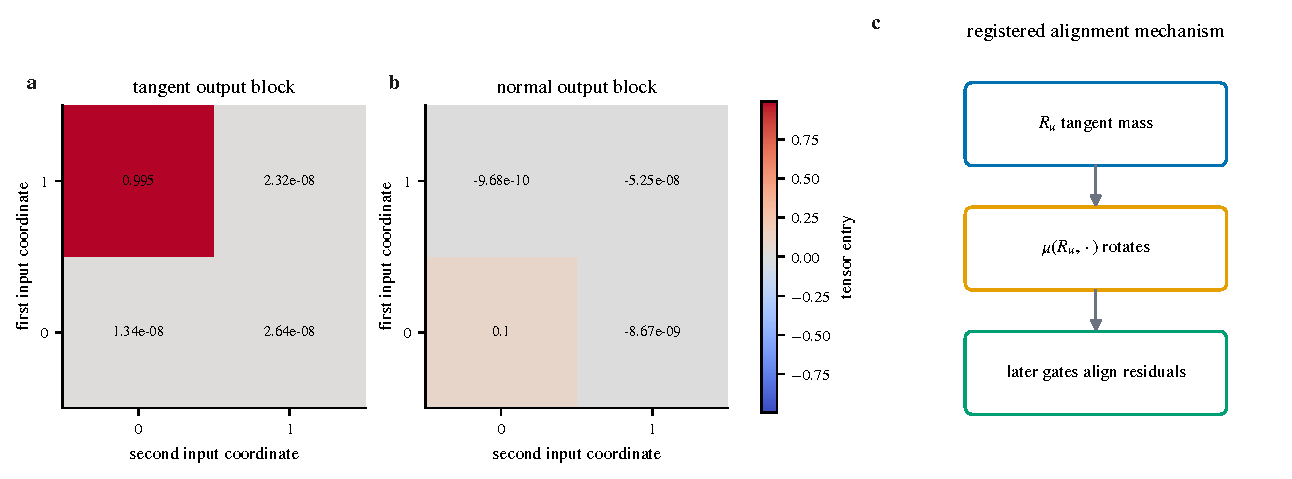
\includegraphics[width=.90\textwidth]{fig11_extremizer_geometry}
\caption{Registered projected-tree extremizer geometry reused from the finite v4 evidence package.}
\end{figure}

\nocite{Yau2016,LodayVallette2012,Higham2002,MooreKearfottCloud2009,EggerEtAl2018,HackbuschTruncation2021}
\bibliographystyle{amsplain}
\bibliography{references}
\end{document}
